
% This LaTeX was auto-generated from MATLAB code.
% To make changes, update the MATLAB code and republish this document.

\documentclass{article}
\usepackage{graphicx}
\usepackage{color}

\sloppy
\definecolor{lightgray}{gray}{0.5}
\setlength{\parindent}{0pt}

\begin{document}

    
    
\subsection*{Contents}

\begin{itemize}
\setlength{\itemsep}{-1ex}
   \item Adam's Bashforth
\end{itemize}
\begin{verbatim}
% Ali Heydari
% Adams-Bashforth Method
% Math 231 Proj 6
\end{verbatim}


\subsection*{Adam's Bashforth}

\begin{verbatim}
% to get CPU time

% desired interval

a = 0;
b = 10;

% size of each step
% h_step = [0.1 0.05];


h_step = [0.1 0.05] ;

% initial value (we have w_1 and w_2 from the Euler's method approximation

w_0 = [1 1 1/10];
w_1 = [0.900000000000000 1  0.180000000000000];
w_2 = [0.811000000000000 0.990000000000000 0.225873075307798];

% the function being solved

f{1} = @(t,x) t^2 - x;
f{2} = @(t,x) -t * x;
f{3} = @(t,x) exp(-2 * t) - 2 * x;

% given solutions
y = cell(3,1);

y{1} = @(t) -1 * exp(-t) + t^2 - 2 * t + 2;
y{2} = @(t) exp(-t^2 / 2);
y{3} = @(t) 1/10 * exp(-2 * t) + t * exp(-2 * t);

% To make our life a lot easier with the plots

str = ["y' = t^2 - y ","y' = -t * y","y' = e^{-2t} - 2y"];


% function call for h = 0.1

[w] = adam_bash_3(a,b,h_step,w_0,w_1,w_2,f,y,str);

% % function call for h = 0.05
% h = 0.05
% [w,error] = euler(a,b,h,w_0,f,y,str);



%
% ylabel(" Log of CPU Time");
% title("Precision Diagram for Adam-Bashforth 3rd order vs Euler's");











function [w] = adam_bash_3(a,b,h_step,w_0,w_1,w_2,f,y,str)

% Number of iterations



% v will be the cell storing the approximated solutions

for k = 1:2

    h = h_step(k);

    N = (b - a) / h;

    % initialization
    w = zeros(N,1);
    t = zeros(N,1);
    v = cell(3,1);


    for i = 1 : 3

        v{i} = zeros (N,1);

    end


    for i = 1 : 3

        % for easier use
        g = f{i};
        w = v{i};
        % initial value, given to us
        w(1) = w_0(i);
        w(2) = w_1(i);
        w(3) = w_2(i);

        for j = 3 : N

            % Euler's
            w(j + 1) = w(j) + h/12 * (23*g(t(j),w(j)) - 16*g(t(j-1),w(j-1))+ ...
                5*g(t(j-2),w(j-2)));

            % to save computaion time, since all the t's will be the same
            % for the consecutive i's
            if i == 1

                t(j + 1) = a + h * j ;

            end

        end

        % storing the current solution
        v{i} = w;


    end

    % initialization
    error = zeros(N,3);
    A = zeros(N,1);

    for  i = 1 : 3

        % for easier use
        g = y{i};
        w = v{i};

        for j = 1 : N

            % evaluating the exact solution at each time
            A(j) = g(t(j));

            % computing the error
            error(j,i) = norm(w(j) - A(j));

            % to get the error at time t == 2

            if h == 0.1

                if j == 20

                    fprintf("For the differential equation %s \n", str(i));
                    fprintf("The error at time = 2 is : %i \n",error(j,i));
                    disp(" ");
                end
            end

            if h == 0.05

                if j == 40

                    fprintf("The error at time = 2 is : %i \n ",error(j,i));


                end

            end

        end


        % plotting stuff
        figure(i);
        hold on



        if k == 1

            plot (t(2:101), A ,'b--o');
            plot (t(2:101),w(1:100),'r');

        end

        if k == 2

            plot (t(1:200),w(1:200),'g');

        end

        xlabel (" Time ");
        ylabel (" y(t) ");
        title ({'Adams-Bashforth: Approximate Solution vs. Actual Solution for : ';  str(i)});
        legend("Actual Solution", "Approximation for h = 0.1",...
            "Approximation for h = 0.05");



        %             xlabel (" Time ");
        %             ylabel (" y(t) ");
        %             title ({'Approximate Solution vs. Actual Solution for : ';  str(i)});
        %             legend("Actual Solution", "Approximation for h = 0.1",...
        %                 "Approximation for h = 0.05");
        %
        %             the error plotsclear
        %             figure(3 + i)
        %             loglog( error(:,i));
        %             title ({'Log-Log Plot of the Error for:';  str(i)})


    end


    %  hold off

end
% returning the final approximations
w = v;

end
\end{verbatim}

        \color{lightgray} \begin{verbatim}For the differential equation y' = t^2 - y  
The error at time = 2 is : 2.328907e-03 
 
Warning: Ignoring extra legend entries. 
For the differential equation y' = -t * y 
The error at time = 2 is : 3.635853e-03 
 
Warning: Ignoring extra legend entries. 
For the differential equation y' = e^{-2t} - 2y 
The error at time = 2 is : 1.671810e-03 
 
Warning: Ignoring extra legend entries. 
The error at time = 2 is : 1.485720e-02 
 The error at time = 2 is : 3.263073e-04 
 The error at time = 2 is : 1.705789e-03 
 \end{verbatim} \color{black}
    
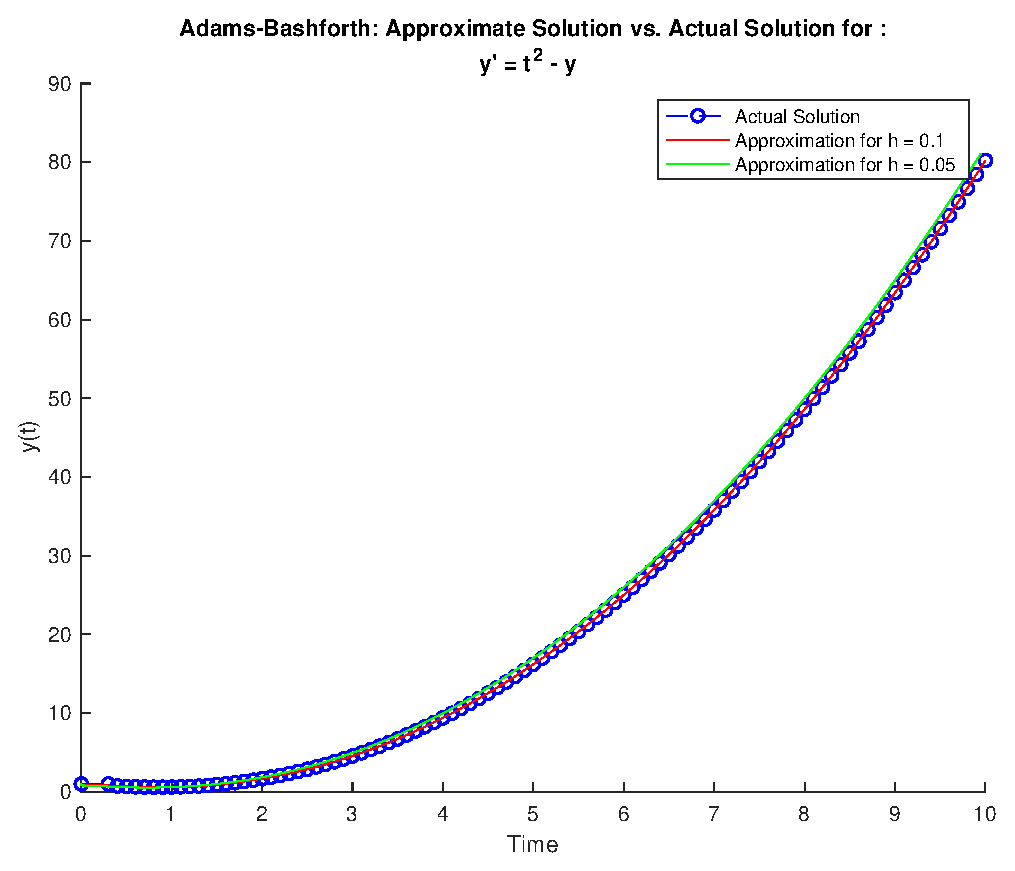
\includegraphics [width=4in]{Adams_bash_3rd_updated_01.eps}

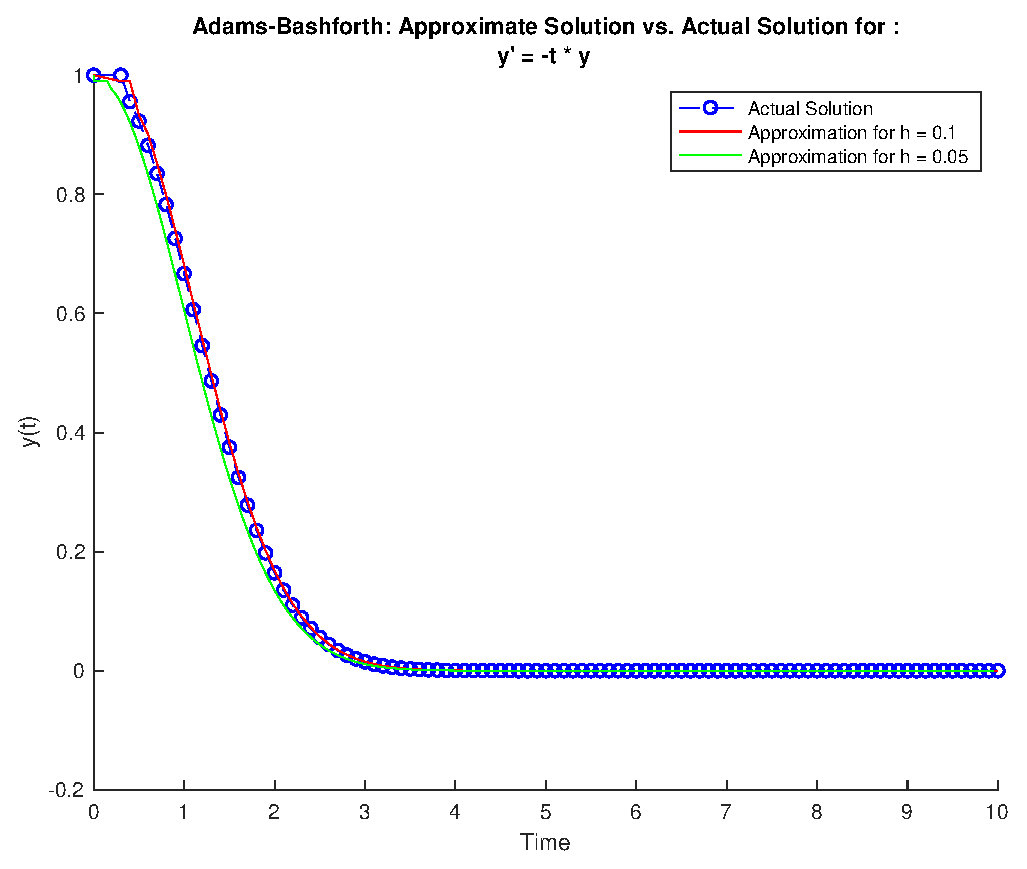
\includegraphics [width=4in]{Adams_bash_3rd_updated_02.eps}

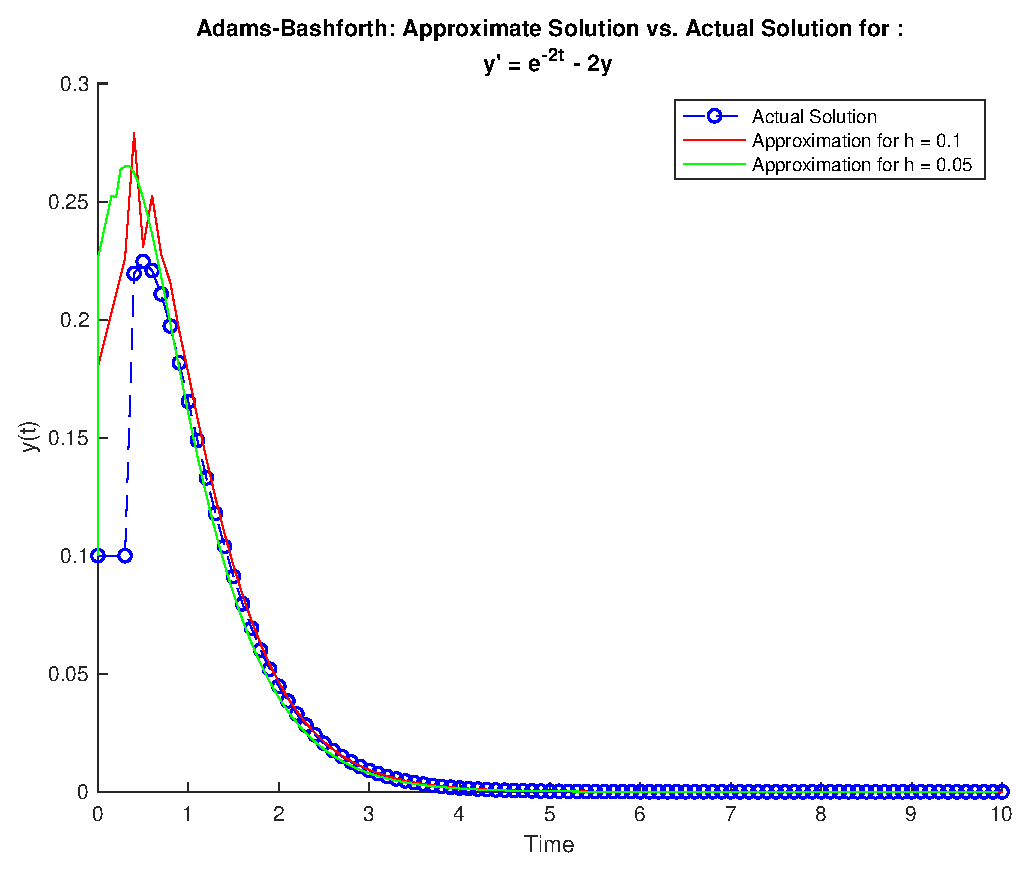
\includegraphics [width=4in]{Adams_bash_3rd_updated_03.eps}



\end{document}
    
